% Created 2019-05-31 Fri 14:14
% Intended LaTeX compiler: pdflatex
\documentclass[12pt]{article}
\usepackage[utf8]{inputenc}
\usepackage[T1]{fontenc}
\usepackage{graphicx}
\usepackage{grffile}
\usepackage{longtable}
\usepackage{wrapfig}
\usepackage{rotating}
\usepackage[normalem]{ulem}
\usepackage{amsmath}
\usepackage{textcomp}
\usepackage{amssymb}
\usepackage{capt-of}
\usepackage{hyperref}
\author{Heitor Lourenço Werneck \\{\href{mailto:heitorwerneck@hotmail.com}{heitorwerneck@hotmail.com}}}
\usepackage[portuguese]{babel}
\usepackage{mathtools}
\usepackage[binary-units=true]{siunitx}
\usepackage[top=0.5cm,bottom=1.5cm,left=2cm,right=2cm]{geometry}
\usepackage{mdframed}
\usepackage{listings}
\usepackage[noend]{algpseudocode}
\usepackage{algorithm}
\usepackage{tikz}
\usepackage[font=small,labelfont=bf]{caption} % Required for specifying captions to tables and figures
\usepackage[subrefformat=parens]{subcaption}
\date{\today}
\title{Algoritmos e Estrutura de Dados III (2019-1)\\\medskip
\large Trabalho Prático 3}
\hypersetup{
 pdfauthor={Heitor Lourenço Werneck},
 pdftitle={Algoritmos e Estrutura de Dados III (2019-1)},
 pdfkeywords={},
 pdfsubject={},
 pdfcreator={Emacs 26.2 (Org mode 9.1.9)}, 
 pdflang={Portuguese}}
\begin{document}

\maketitle
\usetikzlibrary{arrows, fit, matrix, positioning, shapes, backgrounds,intersections}


\newcommand{\algruledefaultfactor}{.75}
\newcommand{\algstrut}[1][\algruledefaultfactor]{\vrule width 0pt
depth .25\baselineskip height #1\baselineskip\relax}
\newcommand*{\algrule}[1][\algorithmicindent]{\hspace*{.5em}\vrule\algstrut
\hspace*{\dimexpr#1-.5em}}

\makeatletter
\newcount\ALG@printindent@tempcnta
\def\ALG@printindent{%
    \ifnum \theALG@nested>0% is there anything to print
    \ifx\ALG@text\ALG@x@notext% is this an end group without any text?
    % do nothing
    \else
    \unskip
    % draw a rule for each indent level
    \ALG@printindent@tempcnta=1
    \loop
    \algrule[\csname ALG@ind@\the\ALG@printindent@tempcnta\endcsname]%
    \advance \ALG@printindent@tempcnta 1
    \ifnum \ALG@printindent@tempcnta<\numexpr\theALG@nested+1\relax% can't do <=, so add one to RHS and use < instead
    \repeat
    \fi
    \fi
}%

\patchcmd{\ALG@doentity}{\noindent\hskip\ALG@tlm}{\ALG@printindent}{}{\errmessage{failed to patch}}

\AtBeginEnvironment{algorithmic}{\lineskip0pt}

\newcommand*\Let[2]{\State #1 $\gets$ #2}
\newcommand*\Stateh{\State \algstrut[1]}

\algnewcommand{\IfThenElse}[3]{% \IfThenElse{<if>}{<then>}{<else>}
  \State \algorithmicif\ #1\ \algorithmicthen\ #2\ \algorithmicelse\ #3}
\algnewcommand{\Break}[0]{\textbf{break}}
\makeatletter
\renewcommand{\ALG@name}{Algoritmo}
\renewcommand{\listalgorithmname}{Lista de\ALG@name s}
\makeatother
\lstset{
  basicstyle=\ttfamily,
  columns=fullflexible,
  frame=single,
  breaklines=true,
  postbreak=\mbox{\textcolor{red}{$\hookrightarrow$}\space},
}
\tikzstyle{block} = [rectangle, draw, 
    text width=5em, text centered]
\tikzstyle{elli} = [draw,ellipse,text width=5em,text centered]
\tikzstyle{decision} = [diamond, draw,text width=4.5em, text badly centered, node distance=3cm, inner sep=0pt]
\tikzstyle{line} = [draw, -latex',dashed]

\newcommand{\myDistance}{2.8cm}
\AtBeginEnvironment{algorithmic}{\footnotesize}
\section{Introdução}
\label{sec:org53f1ac5}
O trabalho a ser apresentado consiste em desenvolver e avaliar soluções ótimas e heurísticas para o problema de coloração de grafos. Uma coloração de k cores de um grafo \(G=(V,E)\), não direcionado, é uma função \(c:V \rightarrow \{1,2,\dots,k\} | (\forall (u,v) \in E) (c(u)\neq c(v))\). O problema de coloração de grafos consiste em determinar o mínimo de cores necessário para colorir um grafo. O menor número de cores utilizado para colorir um grafo é o número cromático de \(G\) que é representado por \(\chi(G)\). Determinar o número cromático de um grafo é conhecido por ser um problema NPC, mais especificamente o seguinte problema de decisão: "Dado um grafo G, \(\chi(G) \leq k\)?". \cite{stockmeyer73_planar_is_polyn_compl,karp72_reduc_combin_probl}

Coloração de grafos e comumente usada em resolução de problemas de agendamento onde há um conjunto \(T\) de trabalhos(todos com o mesmo tempo de realização) que deve ser feito por agentes em alguma maquina. Alguns trabalhos não podem ser feitos no mesmo tempo, porque ele deve ser feito pelo mesmo agente ou pela mesma maquina. Esse problema é basicamente o problema de agendamento em uma escola no qual os agentes são os professores, aulas as maquinas e as disciplinas os trabalhos. \cite{brelaz79_new_method_to_color_vertic_graph}

Outros problemas que a coloração de grafos resolve é alocação de registradores, sudoku e coloração de mapa.

Nesse trabalho será apresentado soluções envolvendo um algoritmo \emph{branch and bound} e duas heurísticas, DSatur e Recursive Largest First(RLF).

\section{Estruturas de dados}
\label{sec:orgf429f9d}

Nesse trabalho existe como objetivo determinar a menor complexidade assintótica de tempo possivel para a solução do problema, para atender a esse parâmetro o grafo é representado como uma matriz de adjacência. Como o grafo desse problema é não ponderado então a estrutura do grafo foi definida como:

\begin{verbatim}
typedef bool weightType;
struct graph{
  int v_qnt;// vertexes
  weightType **adj;// table of edges
};
\end{verbatim}

ou seja o grafo será representado como:

\begin{equation}
\begin{bmatrix}
 v_{11} & v_{12} & \cdots & v_{1j} \\
 v_{21} & v_{22} & \cdots & v_{2j} \\
 \vdots & \vdots & \ddots & \vdots \\
 v_{i1} & v_{i2} & \cdots & v_{ij} \\
\end{bmatrix}
\end{equation}

Com \(v_{ij} \in \{0(\text{Não tem aresta}),1(\text{Existe aresta})\}\) para \(i=1,...,|V| \land j=1,...,|V|\).

Para também ser possível a ordenação do grafo por algum fator sem fazer isomorfismo diretamente no grafo e sim criar uma função que possibilite tal coisa e preservar os nomes dos vértices foi utilizado um tipo de dado que atrela um valor, esse valor foi especificado como grau, ao vértice e tem um campo que guarda seu rótulo fazendo assim o rótulo ser independente do indice de posição do vetor.

\begin{verbatim}
typedef struct vertex{
  int label,degree;
}vertex;
\end{verbatim}


\section{Solução}
\label{sec:orge73f8db}

A primeira solução a ser abordada será a de força bruta com \emph{branch and bound}, esta solução para o problema dará o número cromático do grafo.

\subsection{Branch and bound}
\label{sec:orgee72969}

A solução força bruta com \emph{branch and bound} irá passar pelas possibilidades de coloração evitando buscar soluções onde não será achado uma solução melhor do que a que já se obteve. No pior caso todas possibilidades serão enumeradas se não houver nenhum corte de soluções. O corte se da comparando uma variável que guarda o menor número de cores achados até então, para uma solução, com uma variável que guarda o número de cores usados até então na solução que está sendo construída.

Visto que os algoritmos gulosos dão soluções validas e um limite superior para o número de cores o algoritmo \emph{branch and bound} então pode ser utilizado em conjunto com os algoritmos gulosos delimitando um limite de busca, então se eles derem soluções boas muitos cortes irão ocorrer. Seus algoritmos tem complexidade polinomial como poderá ser visto na seção de análise de complexidade, então são validos pois não irão aumentar a complexidade assintótica, e suas complexidades assintóticas são polinomiais e se poder diminuir o tempo do algoritmo não polinomial ja é algo bom.

No algoritmo \ref{alg:coloringBranchnBound} logo após achar um número máximo de cores é chamado o algoritmo que faz o processo de busca exaustiva com o número máximo de cores para ser feito os cortes.

\begin{algorithm}
\textbf{Input:} G
\textbf{Output:} $\chi \{G \}$
\caption{Branch and bound.}\label{alg:coloringBranchnBound}
\begin{algorithmic}[1]
\Procedure{coloringBranchnBound}{}
\State $maxColor \gets minimum(coloringDSatur(G),coloringRLF(G))$
\State $coloringBranchnBoundR(g,colors,colorsCount,maxColor,0,0)$
\State \Return $maxColor$
\EndProcedure
\end{algorithmic}
\end{algorithm}

O algoritmo de \emph{branch and bound} (algoritmo \ref{alg:coloringBranchnBoundR}) começa verificando se a quantidade de cores utilizadas é maior ou igual ao número minimo de cores utilizado, se for então não é necessário continuar na construção dessa solução pois não dará uma solução melhor que a já obtida logo retorna o número minimo de cores já obtido. Na linha \ref{alg:coloringBranchnBoundR:for1} começa a tentativa de colorir o vértice de \(G.|V|\)(quantidade de vértices de G) cores, primeiro checa se a cor é valida na linha \ref{alg:coloringBranchnBoundR:adjnotsamecolor} se for então colore o vértice(linha \ref{alg:coloringBranchnBoundR:color}).

Depois de colorir o vértice ainda é necessário manter a propriedade da variável \textbf{colorsUsed} que é a de guardar a quantidade de cores utilizadas, basicamente será suposto que em uma solução a maior cor será a quantidade de cores diferentes utilizadas, claro que esse fato elimina algumas outras soluções e também pode dar uma informação errada em uma sequencia de cores do tipo \((1,2,7)\), ou seja na suposição considerada o número de cores diferentes nessa 3-tupla é 7, oque é errado porém sempre há uma solução ótima com essa propriedade, ou seja sempre é possível obter uma solução ótima mesmo com essa suposição feita. Para não ter esse tipo de inconveniência poderia ser calculado o número de cores diferentes em cada chamada porém isso acrescentaria na complexidade de tempo do algoritmo.

Após a manutenção da variável \textbf{colorsUsed} chega a parte de recursão do algoritmo, se chegou no ultimo vértice então retorna o número de cores usadas, se não chegou no ultimo vértice \ref{alg:coloringBranchnBoundR:last} chama a função recursivamente para o próximo vértice, isso irá retornar a quantidade de cores usadas, se a quantidade for menor que a quantidade já obtida então atribui a quantidade de cores mínima.

\begin{algorithm}
\textbf{Input:} G,colors :: refToInteger,colorsCount :: refToInteger,maxColor :: refToInteger,vertex,colorsUsed
\textbf{Output:} $\chi \{G \}$
\caption{Branch and bound recursão.}\label{alg:coloringBranchnBoundR}
\begin{algorithmic}[1]
\Procedure{coloringBranchnBoundR}{}
\If{$*maxColor \leq colorsUsed$}
\State \Return $*maxColor$
\EndIf
\For{$c = 1$ to $G.|V|$}\label{alg:coloringBranchnBoundR:for1}
    \If{$adjNotSameColor(G,colors,c,vertex)$}\label{alg:coloringBranchnBoundR:adjnotsamecolor}
        \State $colors[vertex] = c$\label{alg:coloringBranchnBoundR:color}
	\If{$c>colorsUsed$}
        \State $colorsUsed=c$
	\EndIf

	\If{$vertex+1 < G.|V|$}\label{alg:coloringBranchnBoundR:last}
	    \State $result=coloringBranchnBoundR(G,colors,colorsCount,maxColor,vertex+1,colorsUsed)$
	    \If{$result \neq 0 \land result<*maxColor$}
		\State $*maxColor=result$
	    \EndIf
	\Else
	\State \Return $colorsUsed$
	\EndIf
    \EndIf
\EndFor

\State \Return $*maxColor$
\EndProcedure
\end{algorithmic}
\end{algorithm}

\subsection{DSatur}
\label{sec:org01027fa}
A primeira heurística que foi implementada é o algoritmo DSatur que foi originalmente proposto por Brélaz (1979) \cite{Lewis2016}. A ideia do algoritmo de qual vértice colorir é baseada primeiramente no grau de saturação dos vértices (O grau de saturação de um vértice é o número de cores diferentes nos vértices adjacentes ao mesmo) e seguidamente do grau para ser possível escolher um vértice entre os vértices com maior saturação.

Um fato importante sobre a coloração de grafo é que existe um limite superior bem definido de que \(\chi\{G\}\leq \Delta(G)+1\), onde \(\Delta(G)\) é o grau maximo do grafo G.

No algoritmo \ref{alg:coloringDSatur} é possível ver o funcionamento do algoritmo, primeiro descolore todos vértices e zera a saturação consequentemente. Após isso é calculado o grau de todos vértices que é feito a partir de uma passagem pela matriz de adjacência. Essa matriz de adjacência é ordenada com o método da bolha e depois o vértice com maior grau é colorido. Com o vértice colorido a saturação também deve ser atualizada então o próximo passo é esse, o algoritmo descreve bem esse passo, porém é importante notar o fato que a saturação é feita com base nos índices ordenados através do uso da seguinte expressão para checagem \(vertexList[\textbf{<vértice>}].label\), essa expressão é uma função bijetora \(f: V \rightarrow V^{'}\) , e depois \(saturation[i]\). A consequência do vetor \(saturation\) usar os índices ordenados é que na busca pela maior saturação, no caso de saturações iguais, somente percorrendo o vetor e não parando de pegar uma saturação maior ou igual a maior atual a maior final será a com maior grau das com maior saturação.

Após estes passos começa o processo de construção da solução, esse processo irá passar por todos vértices (linha \ref{alg:coloringDSatur:while}), o primeiro passo é pegar a maior saturação esse é um processo trivial de navegação pelo vetor. O passo de colorir basta criar um vetor que diz se uma cor k existe ou não nos vértices adjacentes e depois achar uma cor que não tenha sido colorida, com a coloração do vértice é necessário atualizar a saturação dos adjacentes a ele com em um laço. A remoção do vértice se da com uma troca do rótulo do vértice para um que sinaliza remoção.

\begin{algorithm}
\textbf{Input:} G
\textbf{Output:} número de cores
\caption{DSatur.}\label{alg:coloringDSatur}
\begin{algorithmic}[1]
\Procedure{coloringDSatur}{}
\For{$i = 0$ to $G.|V|-1$}
   \State $saturation[i] \gets 0$
   \State $colors[i] \gets 0$
\EndFor
\State $vertexList \gets$ Calcula o grau de todos vértices também guardando seu rotulo original
\State $BubbleSort(vertexList)$
\State $colors[vertexList[G.|V|-1].label]=1$\Comment{colore vértice com maior grau}
\For{$i = 0$ to $G.|V|-1$}\Comment{Atualiza saturação}
   \If{$i \neq vertexList[G.|V|-1].label \land G.adj[vertexList[G.|V|-1].label][vertexList[i].label]$}
   \State $saturation[i]\gets saturation[i]+1$
   \EndIf
\EndFor
\While{Não leu todos vértices}\label{alg:coloringDSatur:while}
    \State $vertexLabel \gets maxSaturation(saturation)$\Comment{Pega maior saturação O(G.|V|)}
    \State Colore o vértice com uma cor diferente dos vértices adjacentes
    \State Atualiza saturação dos vértices adjacentes a o normalVertexLabel
    \State Remove o vértice de saturation
\EndWhile
\EndProcedure
\end{algorithmic}
\end{algorithm}

Algumas constatações sobre o algoritmo DSatur é que ele é exato para grafo bipartido, ciclos e roda. \cite{Lewis2016}
A execução do algoritmo é ilustrada na figura \ref{fig:dsaturfuncionamento}.

\begin{center}
\begin{figure}
\begin{subfigure}[b]{.33\linewidth}
\centering
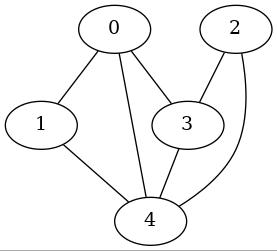
\includegraphics[width=3.3cm]{DSaturFuncionamento1}
\end{subfigure}
\begin{subfigure}[b]{.33\linewidth}
\centering
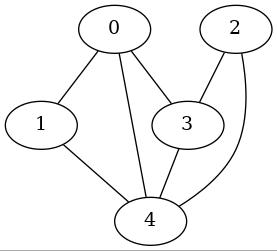
\includegraphics[width=3.3cm]{DSaturFuncionamento2}
\end{subfigure}
\begin{subfigure}[b]{.33\linewidth}
\centering
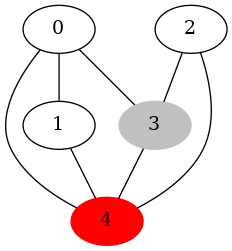
\includegraphics[width=3.3cm]{DSaturFuncionamento3}
\end{subfigure}
\begin{subfigure}[b]{.33\linewidth}
\centering
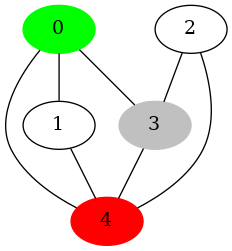
\includegraphics[width=3.3cm]{DSaturFuncionamento4}
\end{subfigure}
\begin{subfigure}[b]{.33\linewidth}
\centering
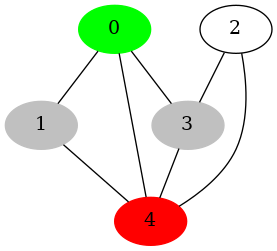
\includegraphics[width=3.3cm]{DSaturFuncionamento5}
\end{subfigure}
\begin{subfigure}[b]{.33\linewidth}
\centering
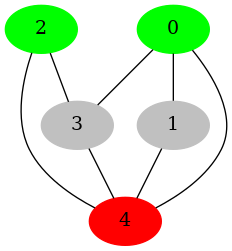
\includegraphics[width=3.3cm]{DSaturFuncionamento6}
\end{subfigure}
\caption{DSatur ilustração da execução.}\label{fig:dsaturfuncionamento}
\end{figure}
\end{center}



\subsection{RLF}
\label{sec:org7da5648}

O algoritmo Recursive Large First(RLF) segue um padrão guloso de construção diferente do DSatur. O RLF foi originalmente feito por Leighton(1979). O algoritmo foca em colorir de uma cor de cada vez, diferente do DSatur que colore um vértice de cada vez.
O algoritmo usa uma heurística para achar um vértice independente e pintar todos vértices desse conjunto independente da mesma cor, após serem coloridos o conjunto independente é removido do grafo. A heurística utilizada para achar o conjunto independente é pegar o vértice de maior grau e depois achar os vértices que não são adjacentes a esse e não são adjacentes entre si.(linha \ref{alg:coloringRLF:u1})

O algoritmo \ref{alg:coloringRLF} mostra o funcionamento.

\begin{algorithm}
\textbf{Input:} G
\textbf{Output:} número de cores
\caption{RLF.}\label{alg:coloringRLF}
\begin{algorithmic}[1]
\Procedure{coloringRLF}{}
\For{$i = 0$ to $G.|V|-1$}
   \State $colors[i] \gets 0$
\EndFor
\State $vertexList \gets$ Calcula o grau de todos vértices também guardando seu rotulo original
\State $remainingVertex \gets G.|V|, c \gets 1$
\While{$remainingVertex>0$}
\State $ChosenVertex\gets higherDegree(vertexList)$
\State $U1 \gets$ Todos vértices não adjacentes a ChosenVertex(incluindo ele mesmo)
\State $U2 \gets vertexList-U1$
\State $U1.grau \gets$ Grau de todos os vértices de $U1$ em relação aos vértices de $U2$
\State $bubbleSort(U1)$
\For{$v$ in $U_{1}$}\label{alg:coloringRLF:for}
\State Checa se algum vértice de $U1$ é adjacente a $v$ e o transfere de $U1$ para $U2$\label{alg:coloringRLF:u1}
\State $colors[v.label]\gets c; vertexList \gets vertexList - v; remainingVertex\gets remainingVertex-1$
\State Decrementa o grau dos vértices adjacentes ao vértice removido
\EndFor
\State $c \gets c + 1$
\EndWhile
\State \Return $c-1$
\EndProcedure
\end{algorithmic}
\end{algorithm}

Um fato sobre o algoritmo RLF é que ele é exato para os mesmos casos que o algoritmo DSatur. A execução do algoritmo é ilustrada na figura \ref{fig:rlffuncionamento}.


\begin{center}
\begin{figure}
\begin{subfigure}[b]{.5\linewidth}
\centering
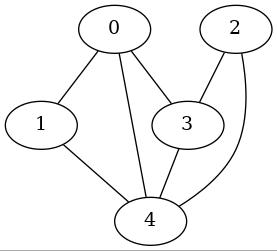
\includegraphics[width=3.3cm]{RLFFuncionamento1}
\end{subfigure}
\begin{subfigure}[b]{.5\linewidth}
\centering
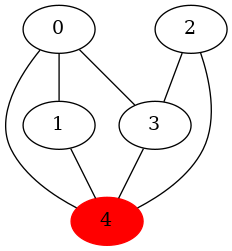
\includegraphics[width=3.3cm]{RLFFuncionamento2}
\end{subfigure}
\begin{subfigure}[b]{.5\linewidth}
\centering
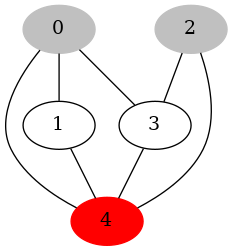
\includegraphics[width=3.3cm]{RLFFuncionamento3}
\end{subfigure}
\begin{subfigure}[b]{.5\linewidth}
\centering
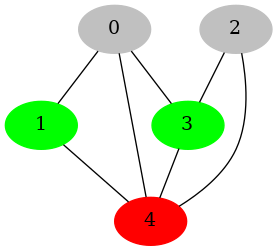
\includegraphics[width=3.3cm]{RLFFuncionamento4}
\end{subfigure}
\caption{RLF ilustração da execução.}\label{fig:rlffuncionamento}
\end{figure}
\end{center}

\section{Análise de complexidade}
\label{sec:org88daed8}
Antes da analise de complexidade é necessário definir alguns termos que darão a complexidade do algoritmo.
\begin{equation}
\underbrace{V}_{\parbox{3.85cm}{quantidade de vértices}}, \underbrace{k}_{\parbox{3.85cm}{quantidade de cores}} \in \mathbb{N}\\
\end{equation}

\subsection{Complexidade de tempo}
\label{sec:orga293be3}
\subsubsection{DSatur}
\label{sec:org578da6b}
O algoritmo \ref{alg:coloringDSatur} faz uso de diversos algoritmos auxiliares que necessitam de análise assintótica. De acordo com o funcionamento de cada componente a complexidade do algoritmo é a seguinte:
\begin{equation}
\begin{aligned}
coloringDSatur(V)\in O(max(V,CalculaGrau,\\BubbleSort,AtualizaSaturacao,V\cdot (maxSaturation + Pinta + AtualizaSaturacao)))\\
CalculaGrau \in O(V^2); BubbleSort \in O(V^2);\\AtualizaSaturacao \in O(V);maxSaturation \in O(V);Pinta \in O(V)\\
coloringDSatur(V)\in O(max(V,V^2,V^2,V\cdot (V + V + V)) \\\therefore coloringDSatur(V)\in O(V^2)
\end{aligned}
\end{equation}


\subsubsection{RLF}
\label{sec:org1e25c8b}
O algoritmo \(coloringRLF\) faz uso de diversos algoritmos auxiliares que necessitam de análise assintótica, alguns iguais ao DSatur.

O laço interno ao "while" do algoritmo tem seus elementos executados \(V\) vezes somente ao invés de \(V^2\), isso pois o conjunto "anda" junto com os vértices remanescentes, logo as funções internas do laço da linha \ref{alg:coloringRLF:for} são executados \(O(V)\) vezes.

De acordo com o funcionamento de cada componente a complexidade do algoritmo é a seguinte:
\begin{equation}
\begin{aligned}
coloringRLF(V)\in O(max(V,CalculaGrau,\\
V\cdot higherDegree,V\cdot ConstrucaoU1U2,V\cdot GrauU1,\\
V\cdot BubbleSort,V\cdot AdjacenteVerifica,V\cdot PintaERemove,\\
V\cdot AtualizaGrau))\\
CalculaGrau \in O(V^2); higherDegree \in O(V);ConstrucaoU1U2 \in O(V);\\GrauU1 \in O(V);AdjacenteVerifica \in O(V);\\ PintaERemove \in O(1);AtualizaGrau \in O(V)\\
coloringRLF(V)\in O(max(V,V^2,V,V^2,V^2,V^3,V^2,V,V^2)) \therefore coloringRLF(V)\in O(V^3)
\end{aligned}
\end{equation}

\subsubsection{Branch and bound}
\label{sec:orgd5d7050}
Uma analise mais intuitiva do algoritmo \emph{branch and bound} é sobre a enumeração das possibilidades, no pior caso do algoritmo ele irá enumerar todas possibilidades de cores. A equação de recorrência do algoritmo \emph{branch and bound} é a seguinte:
\begin{equation}
t(V) = 
\begin{cases}
k\cdot t(V-1) & \text{if $V>1$}\\
k & \text{if $V = 1$}
\end{cases}
\end{equation}

\begin{equation}
\begin{aligned}
t(V)=k\cdot t(V-1)=k^2\cdot t(V-2) = k^{V-1}\cdot t(V-(V-1)) = k^{V-1}\cdot t(1)=k^V
\end{aligned}
\end{equation}
Como o k no algoritmo é sempre a quantidade de arestas então a complexidade será finalmente:
\begin{equation}
\begin{aligned}
k = O(V);
t(V)=k^V; k=V \implies t(V)=V^V
\therefore coloringBranchnBoundR \in O(V^V)
\end{aligned}
\end{equation}
Já a função principal utiliza as heurísticas para ser feito cortes. A complexidade é a mesma complexidade porém é importante incrementar explicitamente essa situação
\begin{equation}
\begin{aligned}
coloringBranchnBound(V) \in O(V^V + coloringDSatur + coloringRLF)\\
O(V^V + V^2 + V^3)\implies coloringBranchnBound(V) \in O(V^V)
\end{aligned}
\end{equation}

A complexidade encontrada é bem ruim no pior caso porém existem algoritmos exatos com complexidade assintótica menor. O melhor algoritmo conhecido para resolver esse problema é o que utiliza o principio de inclusão-exclusão e a transformada Z \cite{bjoerklund09_set_partit_via_inclus_exclus} esse algoritmo tem complexidade \(O(n\cdot 2^n)\).

\subsection{Complexidade de espaço}
\label{sec:org220fcaa}
Antes de se fazer a análise de complexidade de espaço é preciso evidenciar que os algoritmos que possuem em sua lista de parâmetros uma referência para um vetor não apresentará complexidade de espaço relacionada com o espaço ocupado por esse valor referenciado(Ex. \(O(n^c), c \in \mathbb{N}\)) pois o parâmetro guarda uma constante(referência para o vetor) ou seja a complexidade de espaço é constante.\cite{spacecomplexitypointer}

\subsubsection{DSatur}
\label{sec:org30bc95f}
O algoritmo DSatur faz uso de diversas listas para realizar as operações necessarias. Existe uma lista de cores dos vertices, saturação e outros. As funções que o algoritmo chama são todas de complexidade \(O(1)\). Logo como faz uso de listas de uma dimensão somente então a complexidade do algoritmo \ref{alg:coloringDSatur} é \(O(V)\) pois o grafo é passado com complexidade constante para a função por ser uma referencia. Porém no contexto geral desse algoritmo no programa principal sua complexidade pode ser vista como \(O(V^2)\).

\subsubsection{RLF}
\label{sec:orge540cfc}
O algoritmo RLF faz uso também de diversas listas como o DSatur, todas elas unidimensionais e todas função auxiliares chamadas tem complexidade de espaço \(O(1)\) então a complexidade do algoritmo \ref{alg:coloringRLF} é \(O(V)\). Porém assim como o DSatur em um contexto geral sua complexidade pode ser vista como \(O(V^2)\).

\subsubsection{Branch and bound}
\label{sec:orgd4f917d}

A complexidade de espaço do algoritmo \ref{alg:coloringBranchnBoundR} está atrelada a sua recursão pois existe um custo de guardar o contexto atual a cada chamada, na lista de parâmetros todas as variaveis tem custo \(O(1)\) e o algoritmo no máximo guarda os parâmetros V vezes devido a seu comportamento recursivo, logo a complexidade do algoritmo é \(O(V)\).

\subsection{Análise geral}
\label{sec:orgd7b1c3c}

A tabela \ref{tab:org541b157} mostra todas complexidades obtidas, com ela pode-se ver que o melhor algoritmo é o DSatur em questão de complexidade assintótica de tempo e o pior é o \emph{branch and bound}. No geral também pode-se ver que todos algoritmos tem a mesma complexidade de espaço logo nenhum deles tem alguma vantagem sobre o outro nesse quesito.

O programa principal necessita de alocar a matriz de adjacência que representa o grafo, isso tem custo \(O(V^2)\).
\begin{table}[htbp]
\centering
\begin{tabular}{lll}
\hline
Complexidade & Tempo & Espaço\\
\hline
DSatur & \(O(V^2)\) & \(O(V)\)\\
RLF & \(O(V^3)\) & \(O(V)\)\\
Branch and bound & \(O(V^V)\) & \(O(V)\)\\
Principal & \(O(V^V + V^2 + V^3)\) & \(O(V^2)\)\\
\hline
\end{tabular}
\caption{\label{tab:org541b157}
Complexidades.}

\end{table}


\section{Resultados}
\label{sec:orgf04e3b4}

A maquina utilizada para os experimentos possui as seguintes especificações: Intel(R) Core(TM) i3-4005U CPU @ 1.70GHz e 4GiB de memória RAM.

\subsection{Tempo}
\label{sec:org90c8c34}
Antes da análise de resultados é importante refletir sobre quais fatores influenciam no tempo de execução. Nesse caso há os vértices e arestas. Primeiro então é necessario observar como o tempo se comporta com a variação desses parâmetros. È fato que também a maneira que as arestas estão dispostas afetam no tempo porém a analise desse fator é muito complexa e não será abordada.

Na figura \ref{fig:vertice-aresta-a} o algoritmo força bruta parece ter o maior tempo de execução quando o número de arestas esta proximo de 87\% da capacidade total. Já o DSatur e RLF, de acordo com a figura \ref{fig:vertice-aresta-b}, aumentam seu tempo quando o número de arestas se aproxima de 55\%.

\begin{center}
\begin{figure}
\begin{subfigure}[b]{.49\linewidth}
\centering
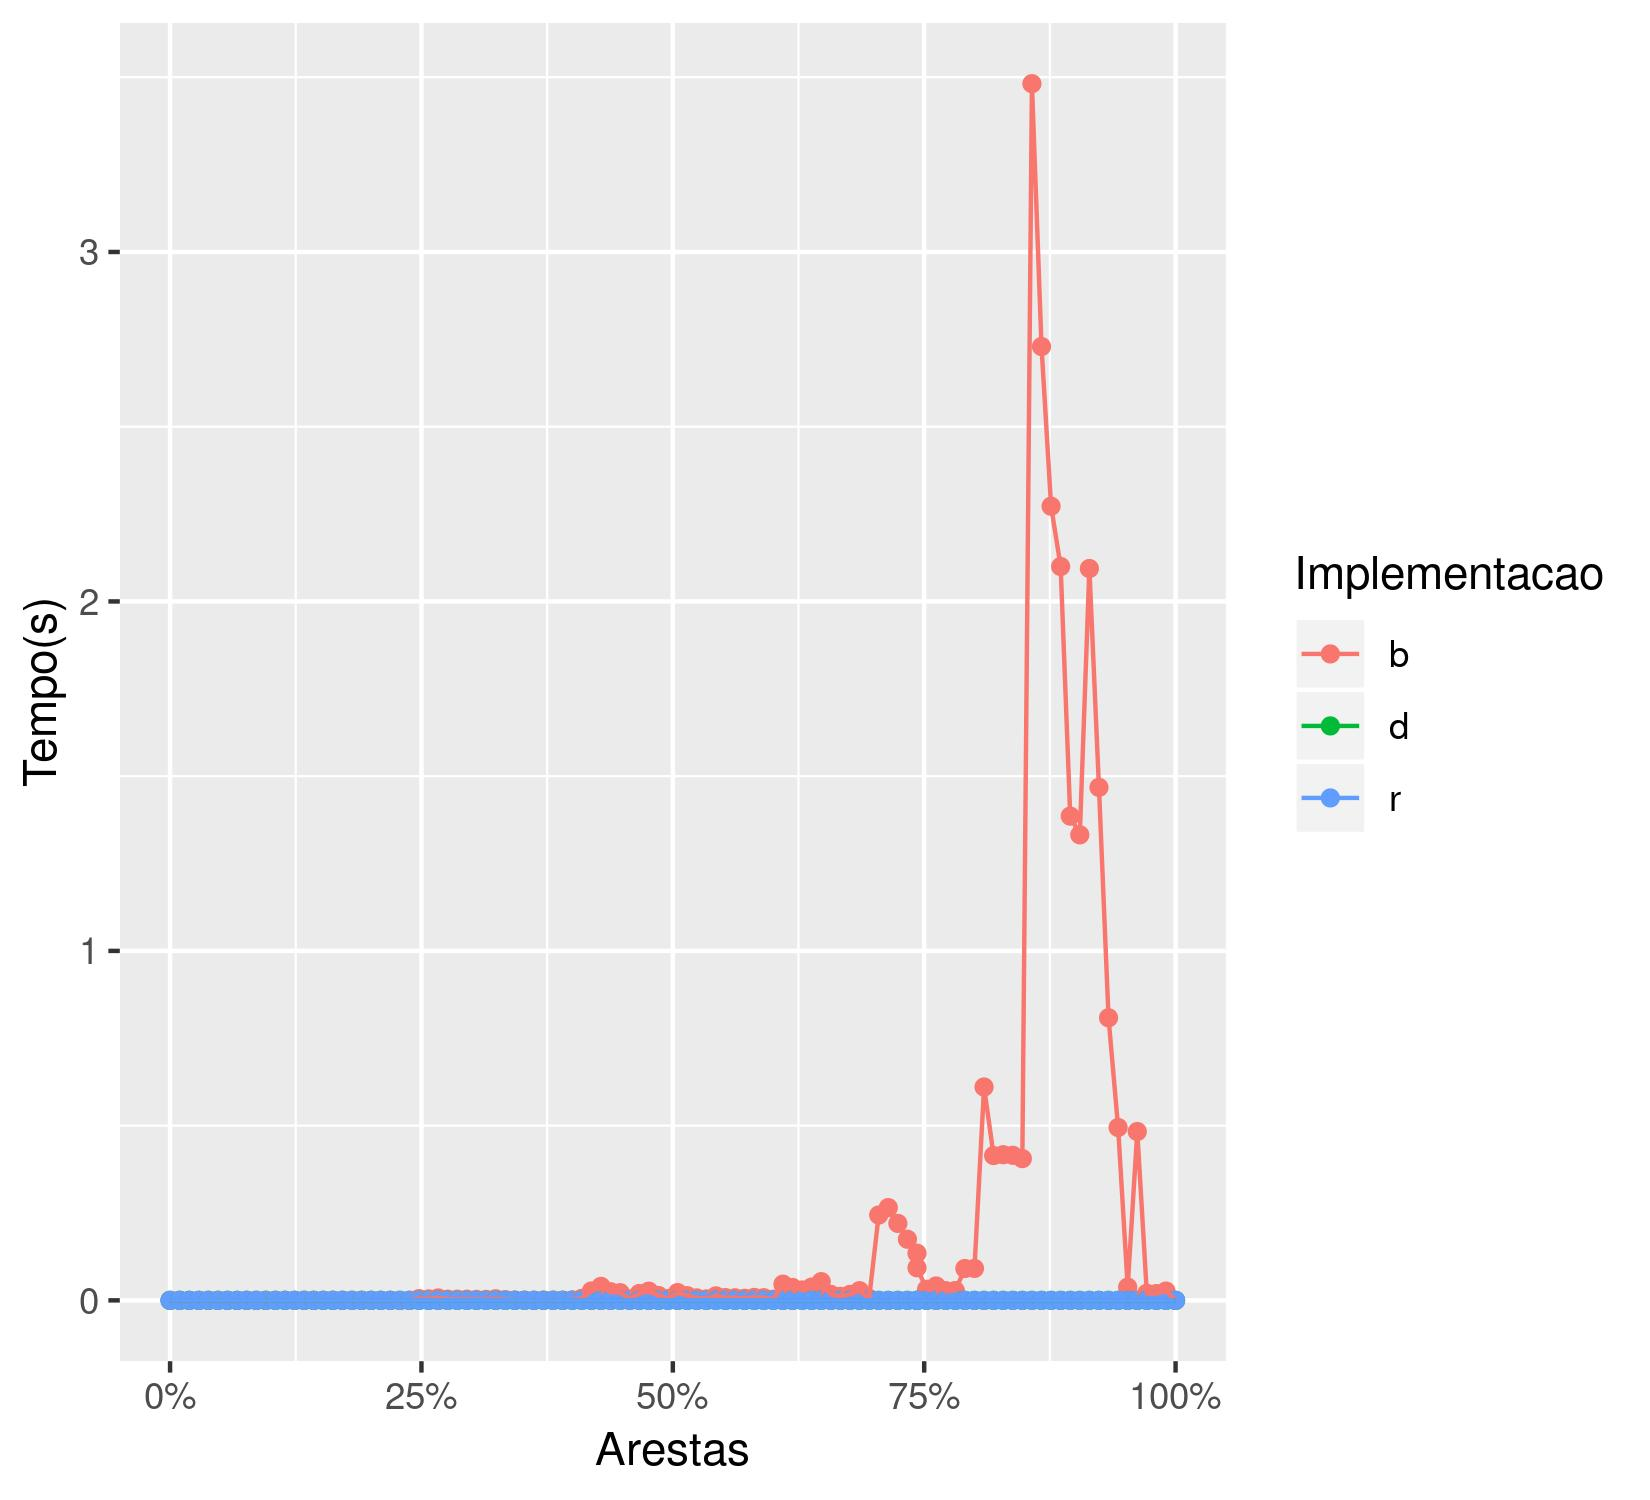
\includegraphics[width=7.5cm]{vertice-aresta-a}
\caption{Branch and bound e outros.}\label{fig:vertice-aresta-a}
\end{subfigure}
\begin{subfigure}[b]{.49\linewidth}
\centering
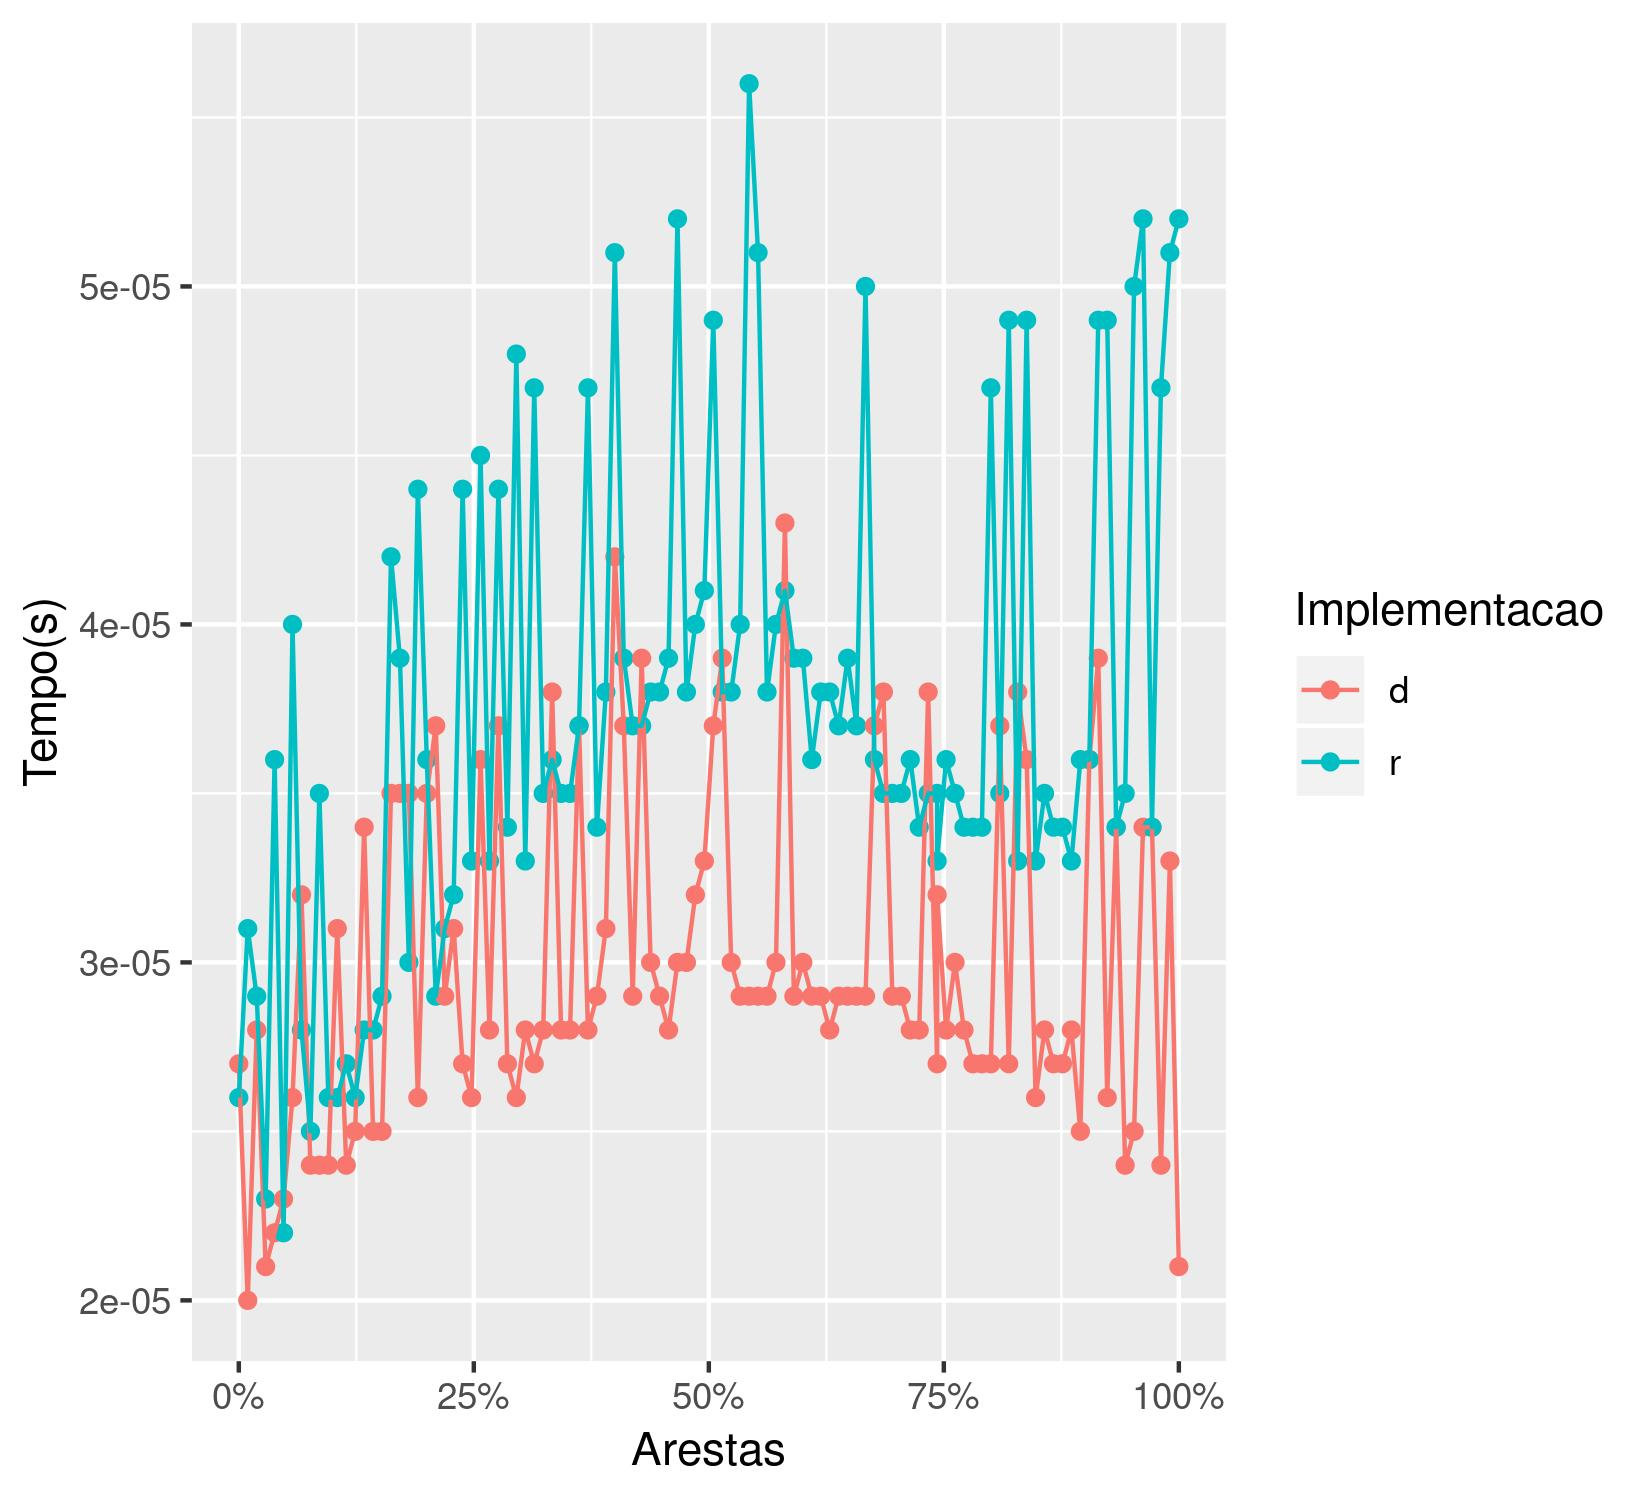
\includegraphics[width=7.5cm]{vertice-aresta-b}
\caption{DSatur e RLF.}\label{fig:vertice-aresta-b}
\end{subfigure}
\caption{Crescimento de acordo com variação de arestas com disposição aleatória(15 vértices).}\label{fig:vertice-aresta}
\end{figure}
\end{center}

Agora para verificar se as complexidades obtidas que estão na tabela \ref{tab:org541b157} são corretas é preciso gerar entradas que exploram o pior caso para obter o pior tempo. Com base no pior tipo de conteúdo em uma entrada, que acabou de ser descoberto, de cada algoritmo, basta variar o número de vertices.

A regressão feita no algoritmo \emph{branch and bound}, como pode ser visto na figura \ref{fig:regressaobnb}, é melhor que a complexidade obtida na tabela \ref{tab:org541b157}, isso pois o valor \(3.78\) da função \(f(x)=3.78^{x-13.88}\) é uma constante e mesmo assim a regressão funcionou. Isso mostra que o \emph{branch and bound} é um bom algoritmo dentre algoritmos exatos, pois um tentativa e erro não cortaria tantas soluções como o branch and bound é capaz. O maior valor obtido foi com 19 vértices e um tempo de \(902.958661\) segundos. Para uma entrada 10 vezes maior o tempo necessário será de \(5.10335e101\) segundos.

Na figura \ref{fig:regressaord} há a regressão dos outros dois algoritmos. O algoritmo DSatur foi comprovado sua complexidade \(O(V^2)\). Já o algoritmo RLF mostrou uma complexidade assintótica melhor que a esperada de \(O(V^3)\) porém como observado em \cite{Leighton_1979} o algoritmo se comporta como \(O(V^2)\) para colorir grafos que \(k\times E \approx V^2\), onde \(E\) é o numero de arestas.

\begin{center}
\begin{figure}
\begin{subfigure}[b]{.49\linewidth}
\centering
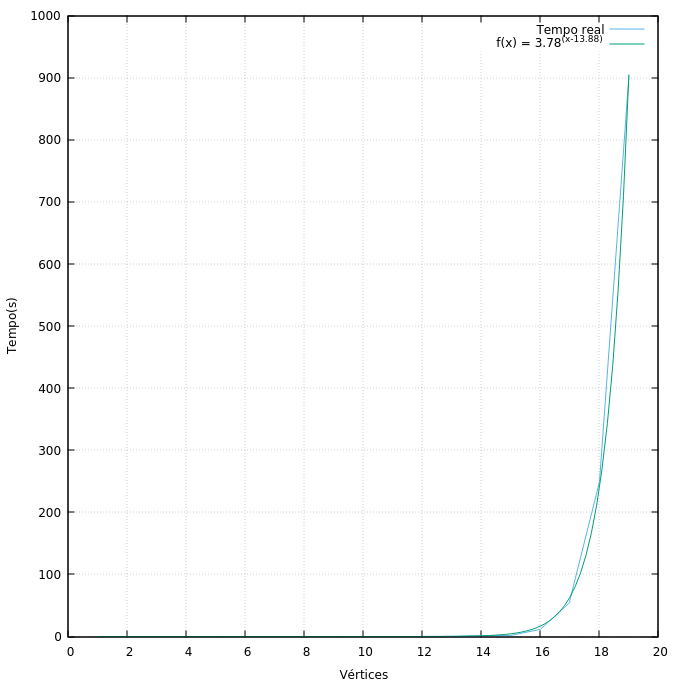
\includegraphics[width=7.5cm]{regressaobnb}
\caption{Branch and bound.}\label{fig:regressaobnb}
\end{subfigure}
\begin{subfigure}[b]{.49\linewidth}
\centering
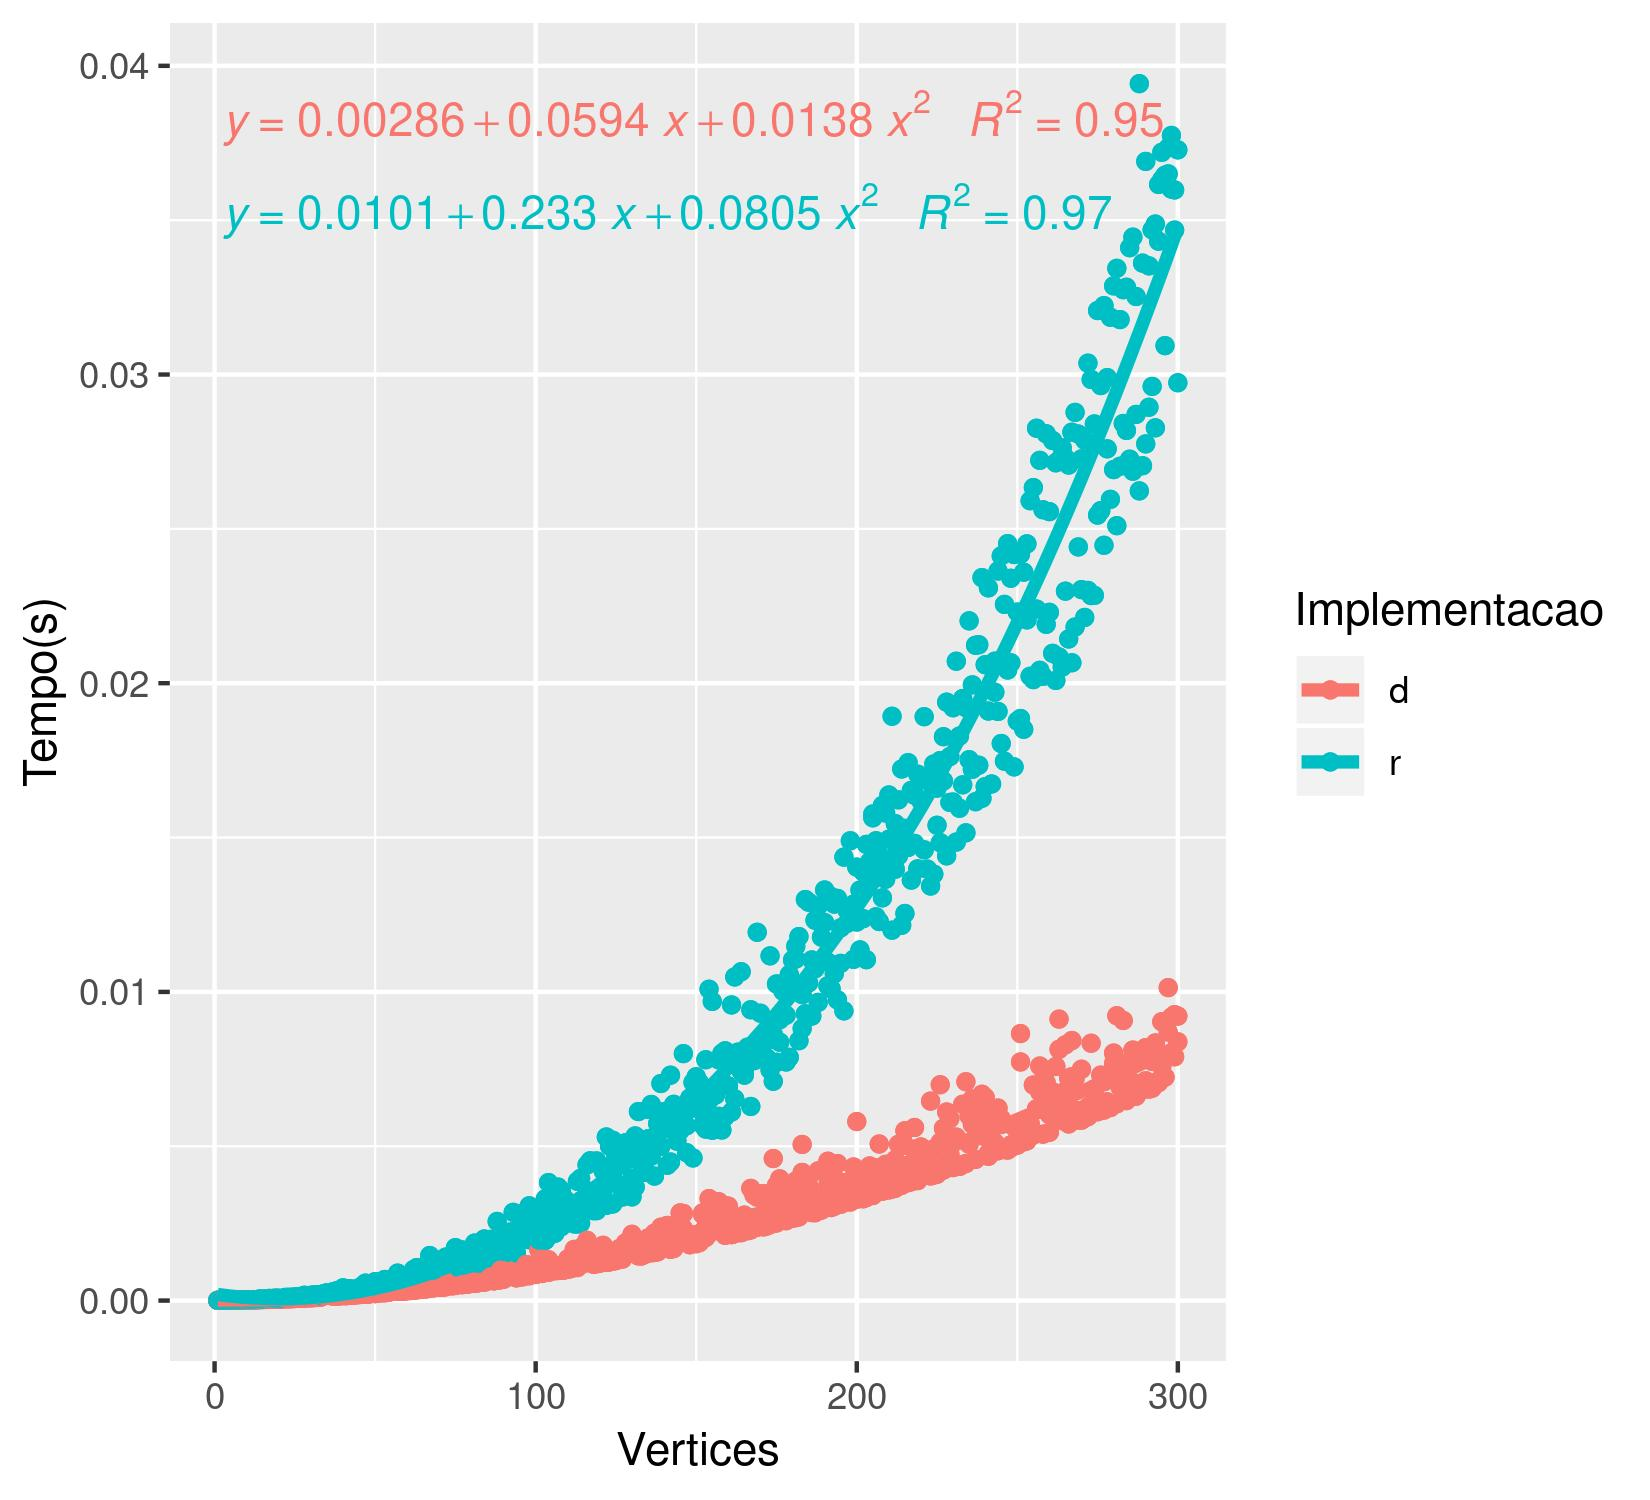
\includegraphics[width=7.5cm]{regressaord}
\caption{DSatur e RLF.}\label{fig:regressaord}
\end{subfigure}
\caption{Complexidade de tempo, regressão.}
\end{figure}
\end{center}

\subsection{Espaço}
\label{sec:org6622c04}

Para provar a complexidade de espaço do algoritmo principal basta monitorar as alocações feitas pelo algoritmo para cada tamanho de entrada. O monitoramento será feito somente da memória \emph{heap} \cite{osthreeeasypieces} que é a parte da memória onde a alocação dinâmica é feita e o espaço pode-se variar dinamicamente permitindo-se assim obter uma função de complexidade correta.

Pela figura \ref{fig:espaco} o espaço utilizado pelos 3 algoritmos foi comprovado e como dito os 3 algoritmos tem regressões polinomiais parecidas que provém do algoritmo principal na alocação de memória para o grafo de entrada(matriz de adjacência).
Isso fica óbvio vendo que o fator do termo de ordem 2 é igual para todos algoritmos e é essa uma parte da quantidade de memória usada pelo programa principal.

\begin{figure}[htbp]
\centering
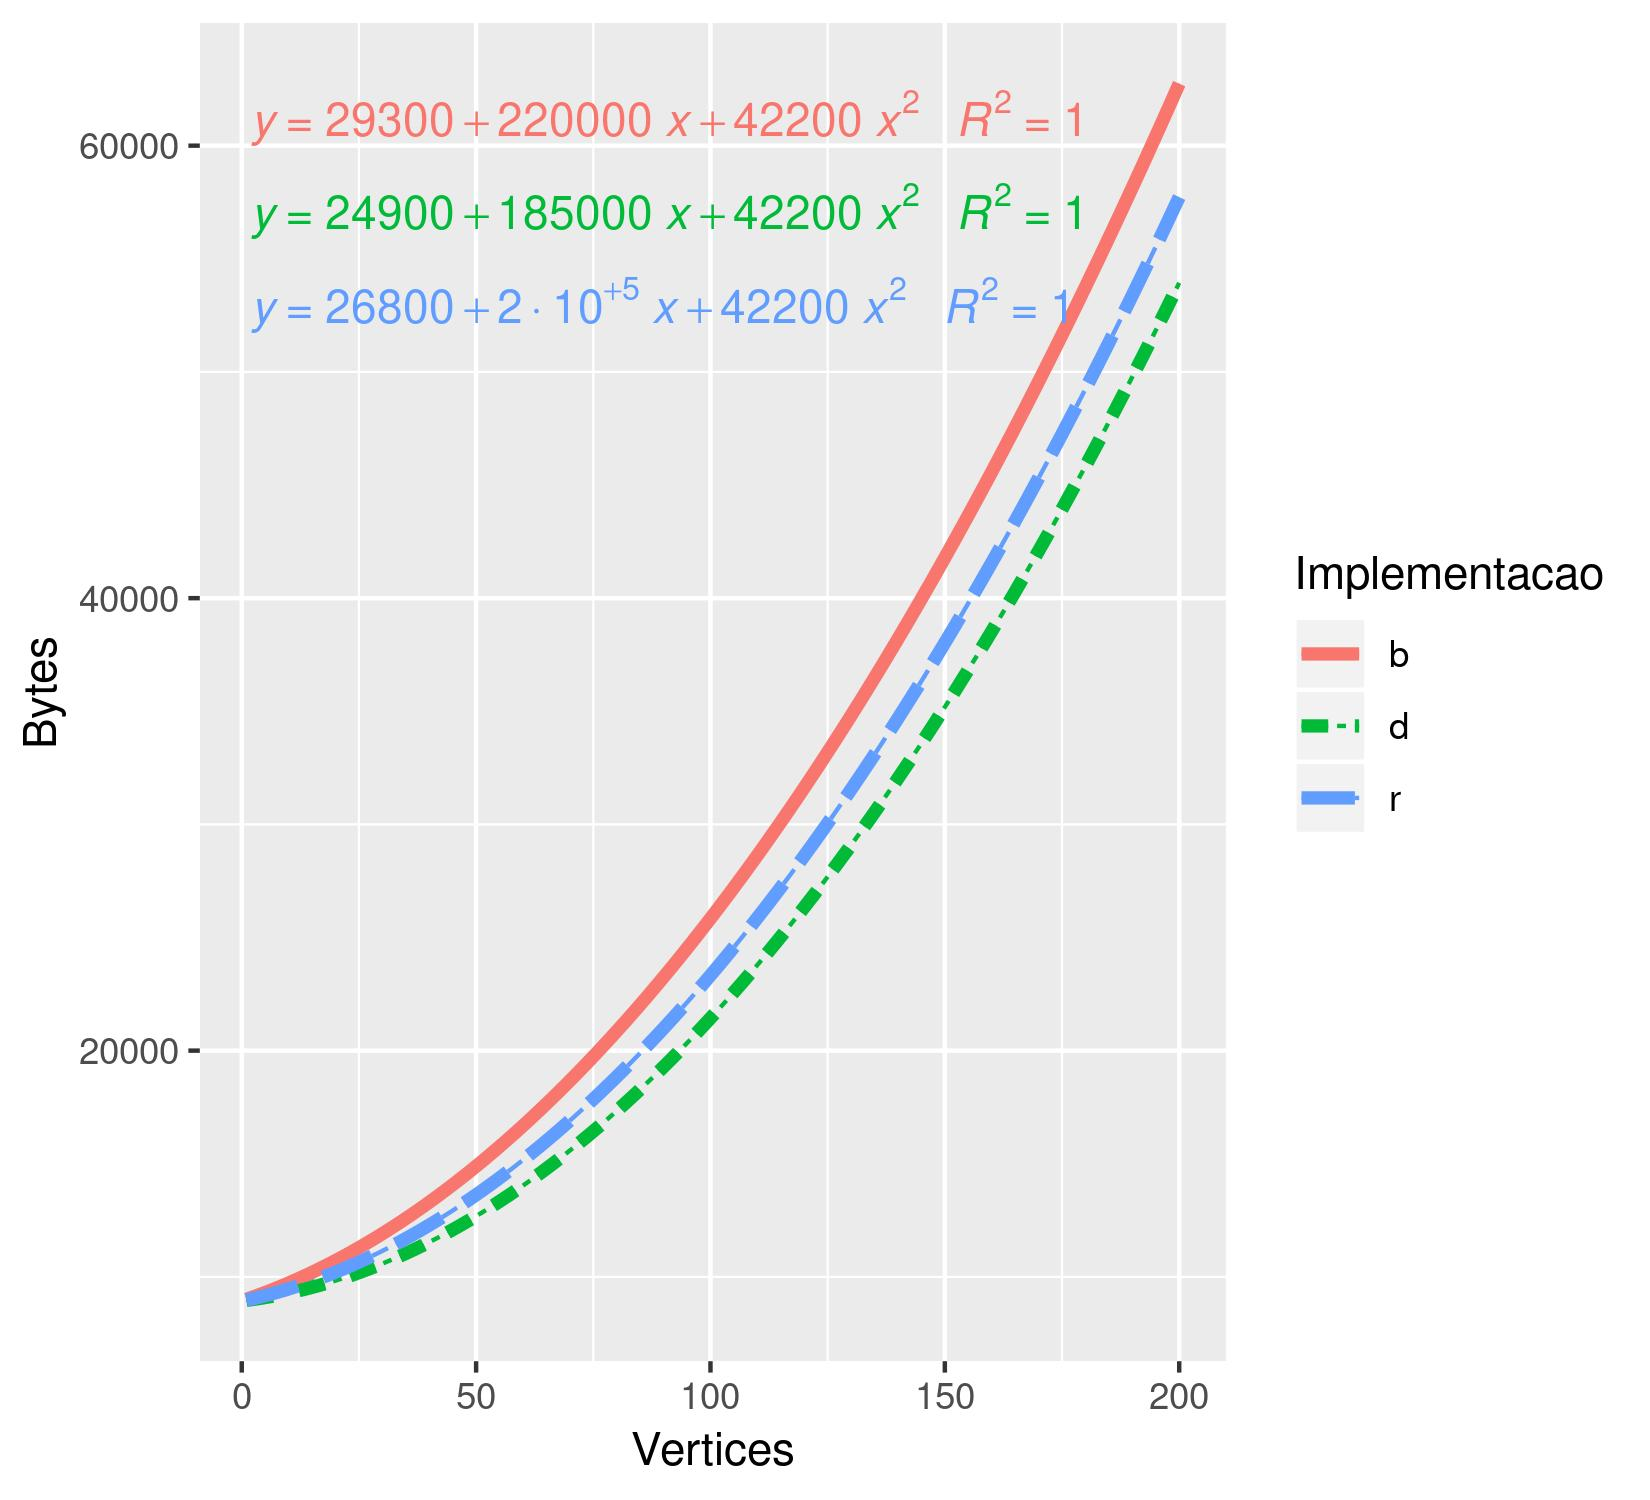
\includegraphics[width=0.33\textwidth]{espaco.jpg}
\caption{Espaço usado pelos algoritmos.\label{fig:espaco}}
\end{figure}

\subsection{Estrategia gulosa}
\label{sec:org5098f28}

A taxa de acerto das heurísticas é mostrado na figura \ref{fig:greedy-ac}, com uma quantidade pequena de vértices o algoritmo achou a solução ótima nesses gráficos porém com o aumento de vértices a solução piora ou pelo menos a incerteza aumenta. O algoritmo RLF apresenta uma taxa de acerto alta, já o algoritmo DSatur dá soluções que tem 50\% de erro(figura \ref{fig:barplot-greedy}) nesses casos aleatorizados. Porém é importante notar que a taxa de acerto pode variar com o tipo do problema(disposição das arestas).

\begin{center}
\begin{figure}
\begin{subfigure}[b]{.49\linewidth}
\centering
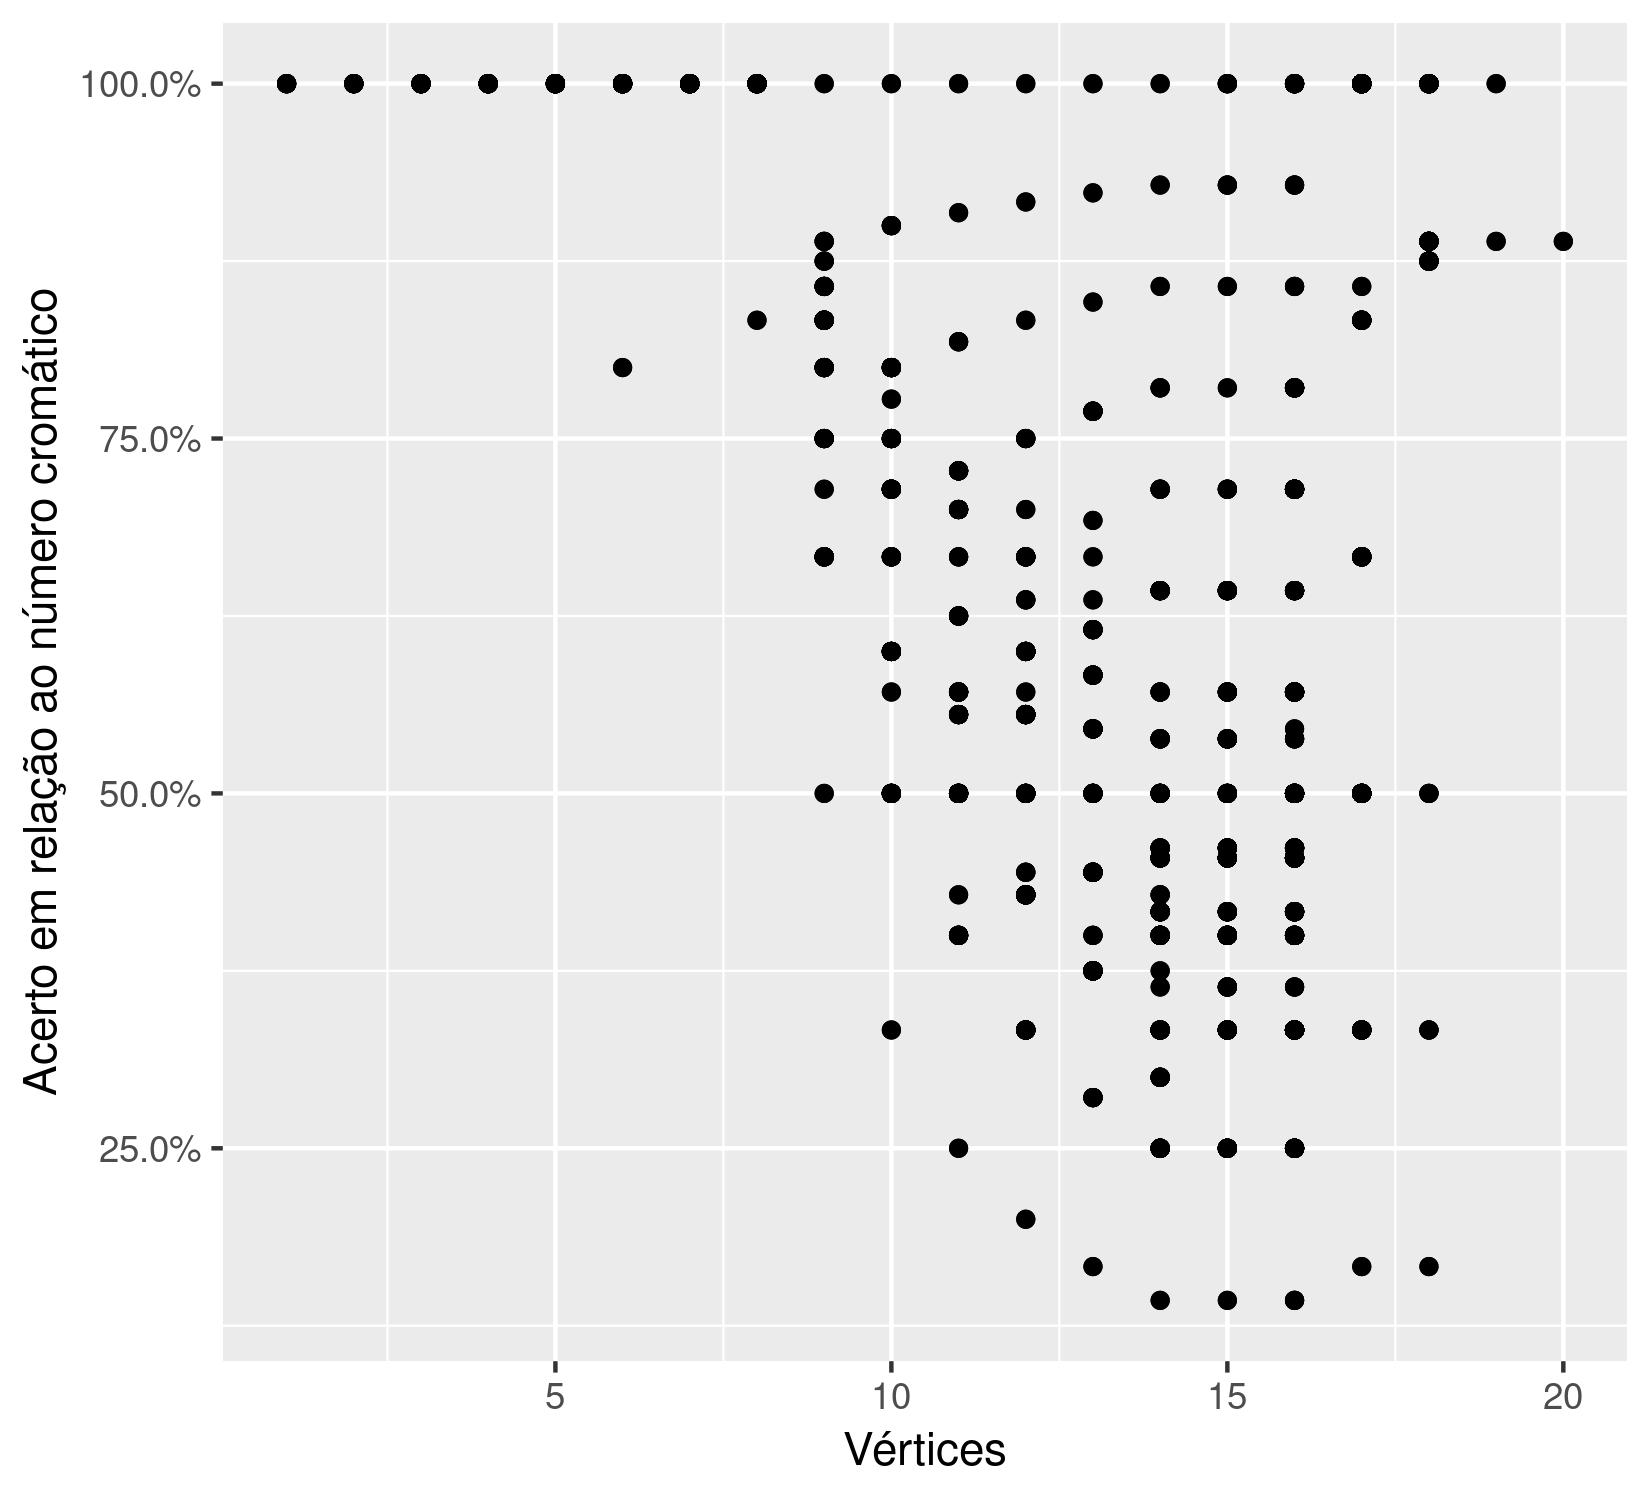
\includegraphics[width=\linewidth/2]{greedy-ac-d}
\caption{DSatur.}\label{fig:greedy-ac-d}
\end{subfigure}
\begin{subfigure}[b]{.49\linewidth}
\centering
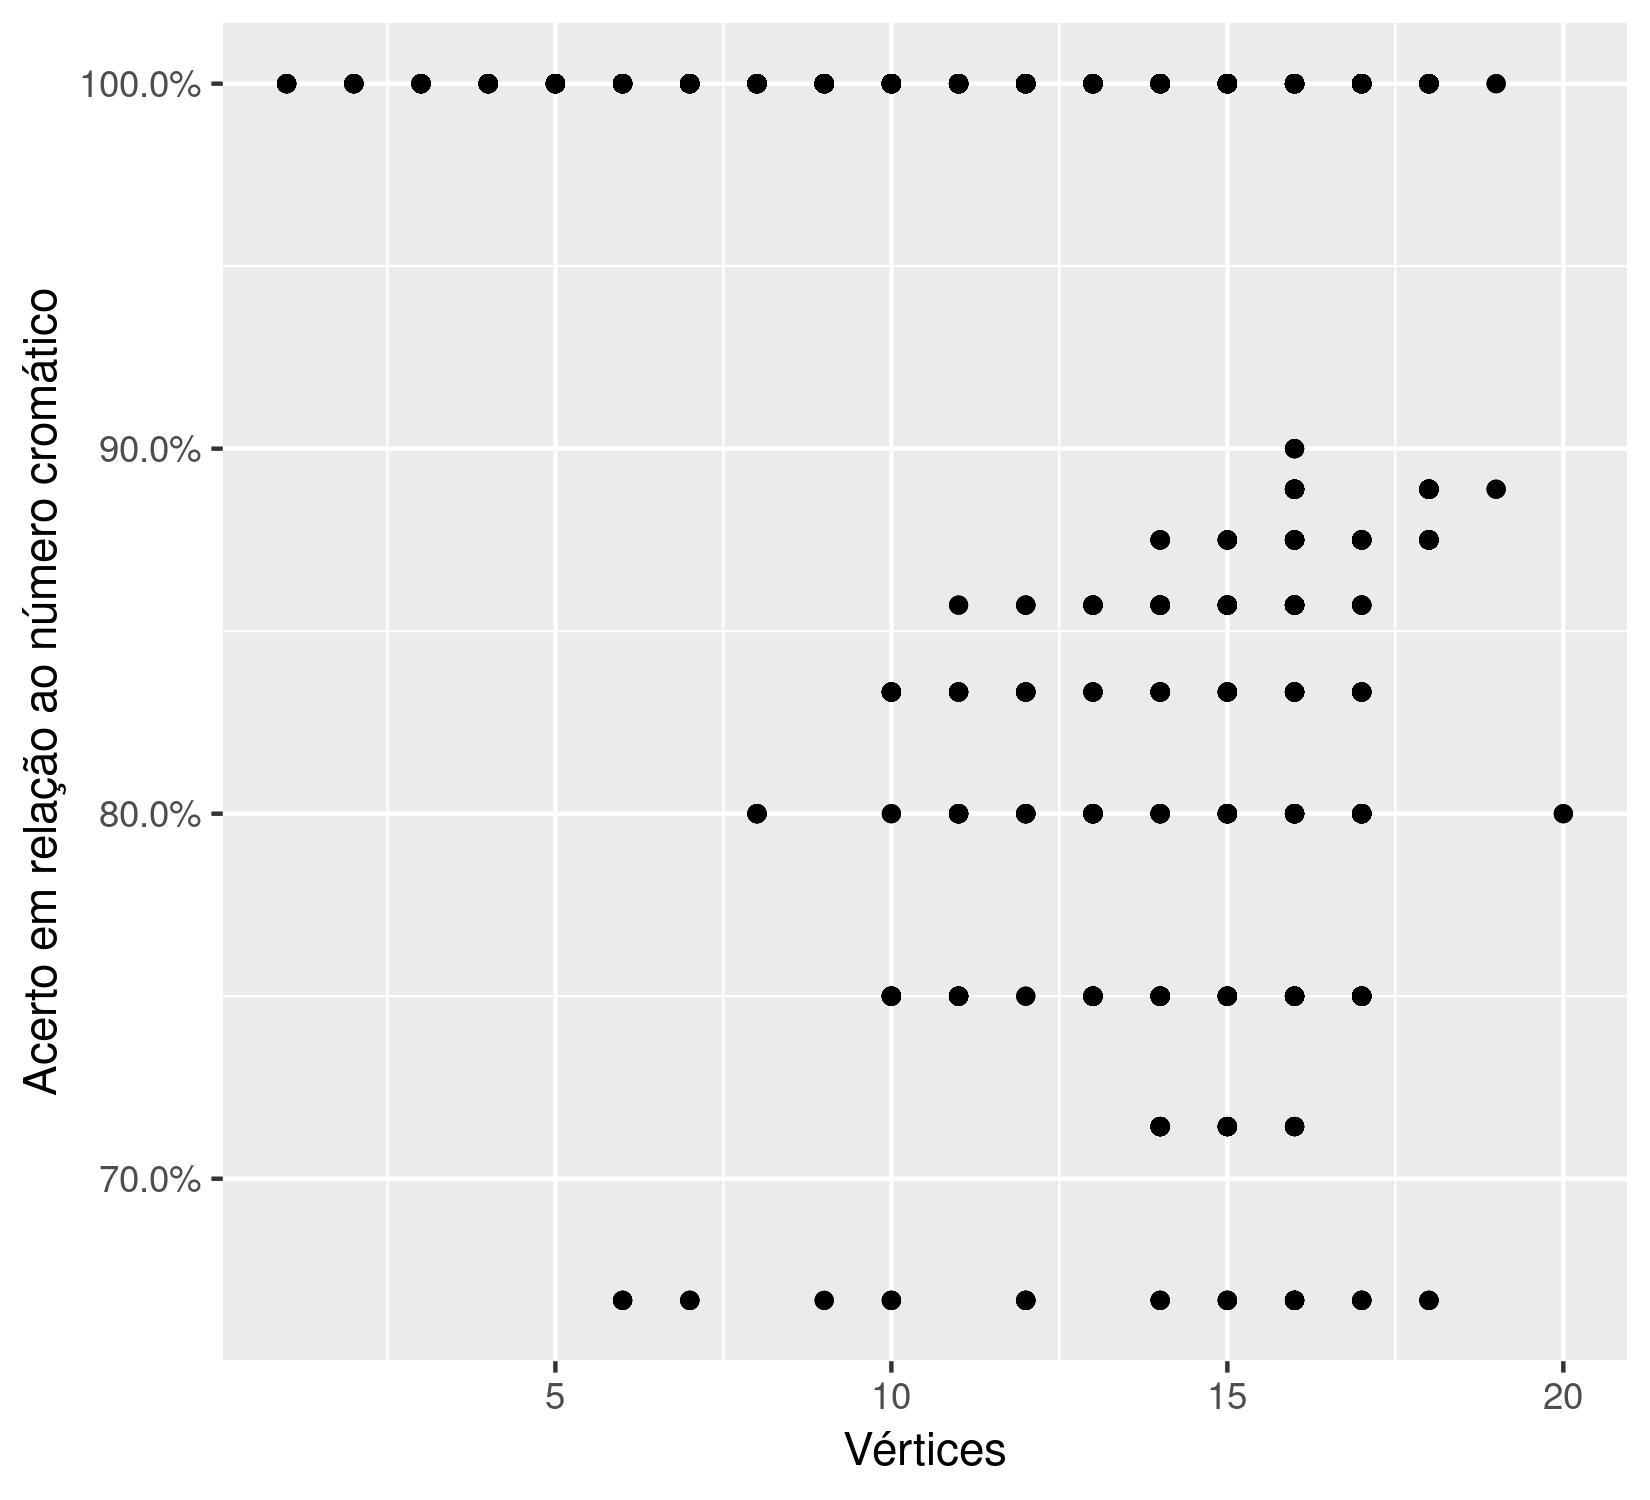
\includegraphics[width=\linewidth/2]{greedy-ac-r}
\caption{RLF.}\label{fig:greedy-ac-r}
\end{subfigure}
\caption{Taxa de acerto das heurísticas.}\label{fig:greedy-ac}
\end{figure}
\end{center}


\begin{center}
\begin{figure}
\begin{subfigure}[b]{.49\linewidth}
\centering
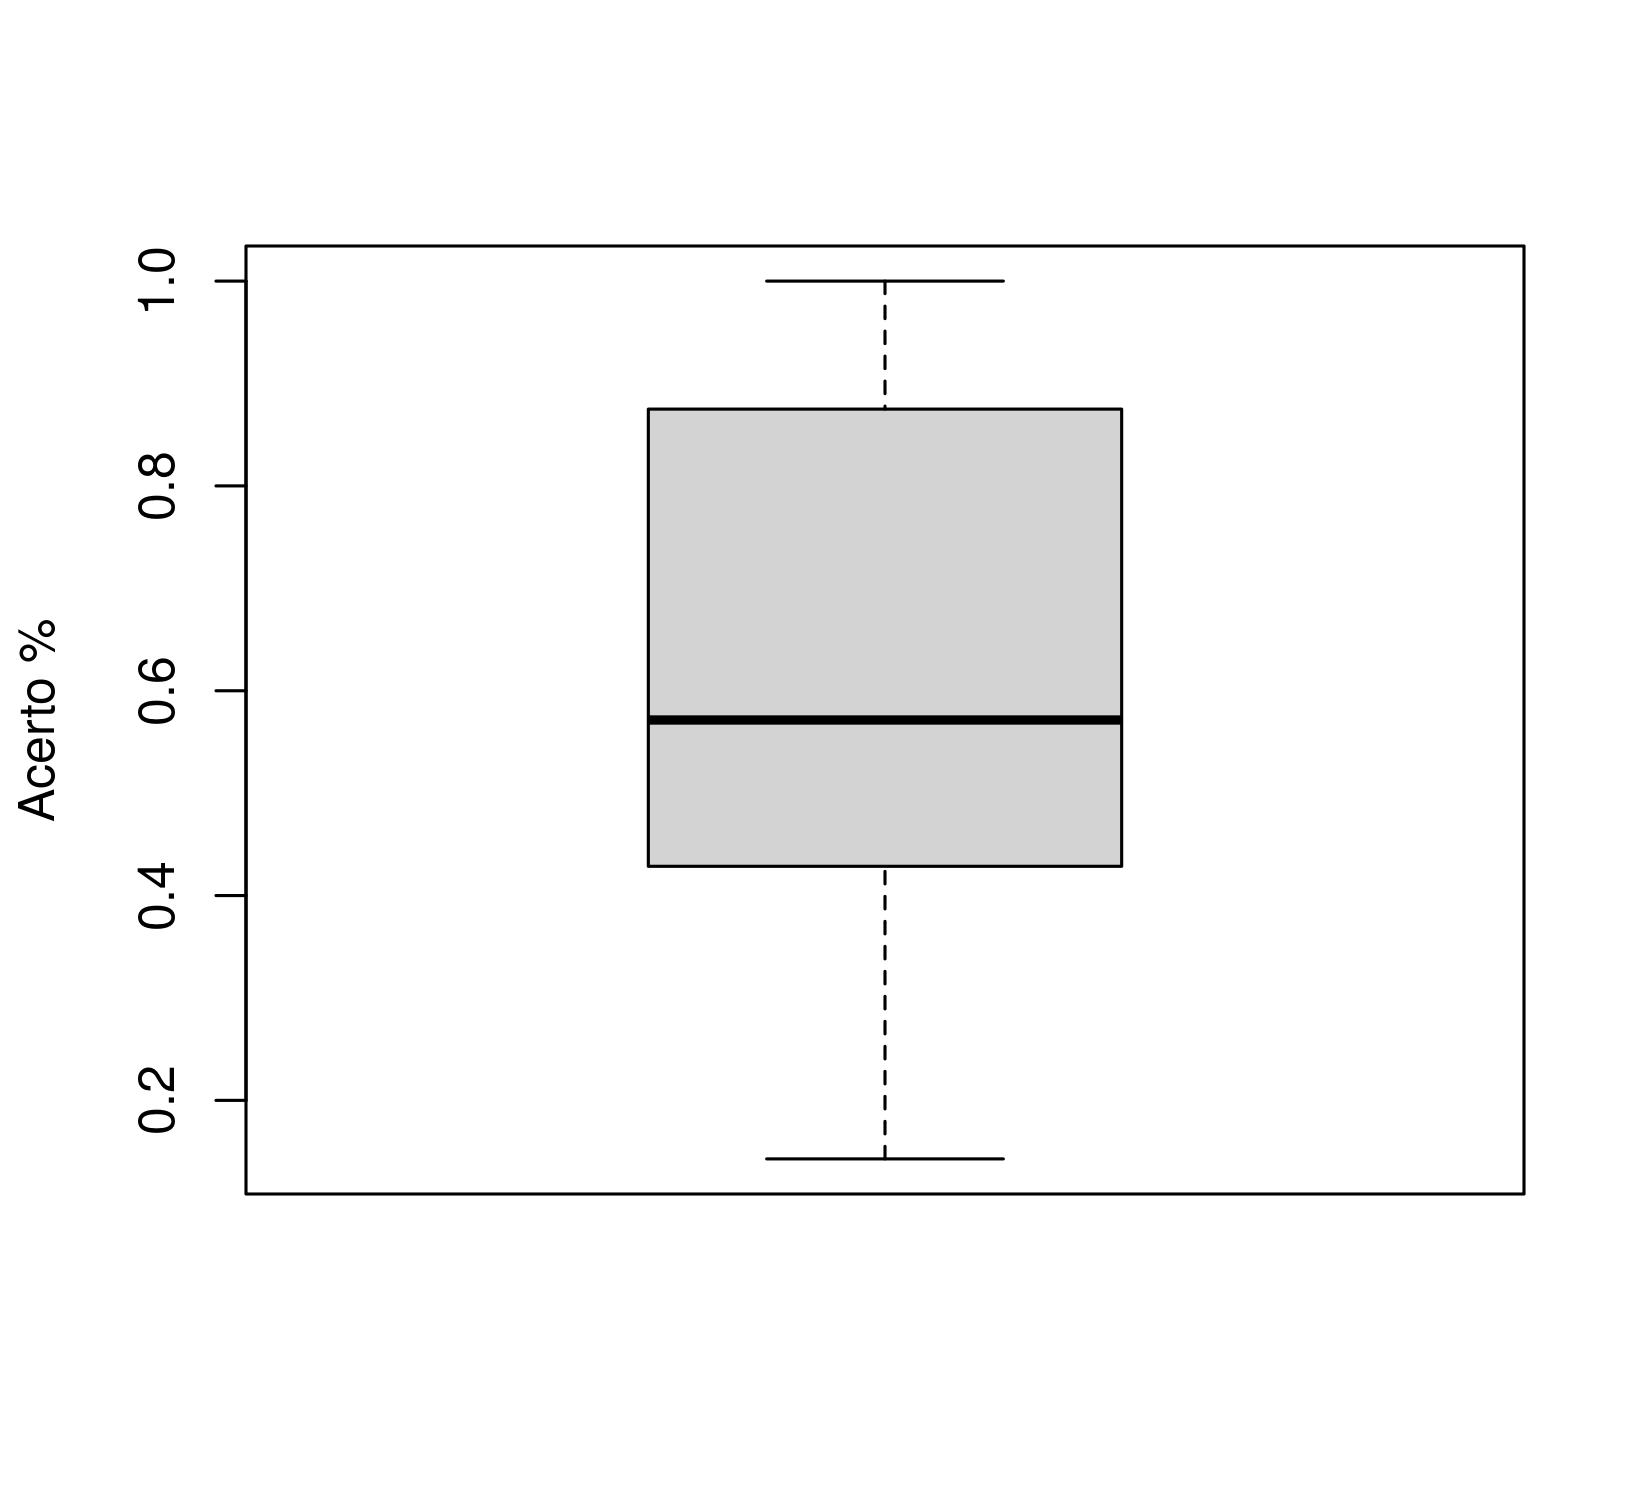
\includegraphics[width=\linewidth/2]{bar-greedy-ac-d}
\caption{DSatur.}\label{fig:bar-greedy-ac-d}
\end{subfigure}
\begin{subfigure}[b]{.49\linewidth}
\centering
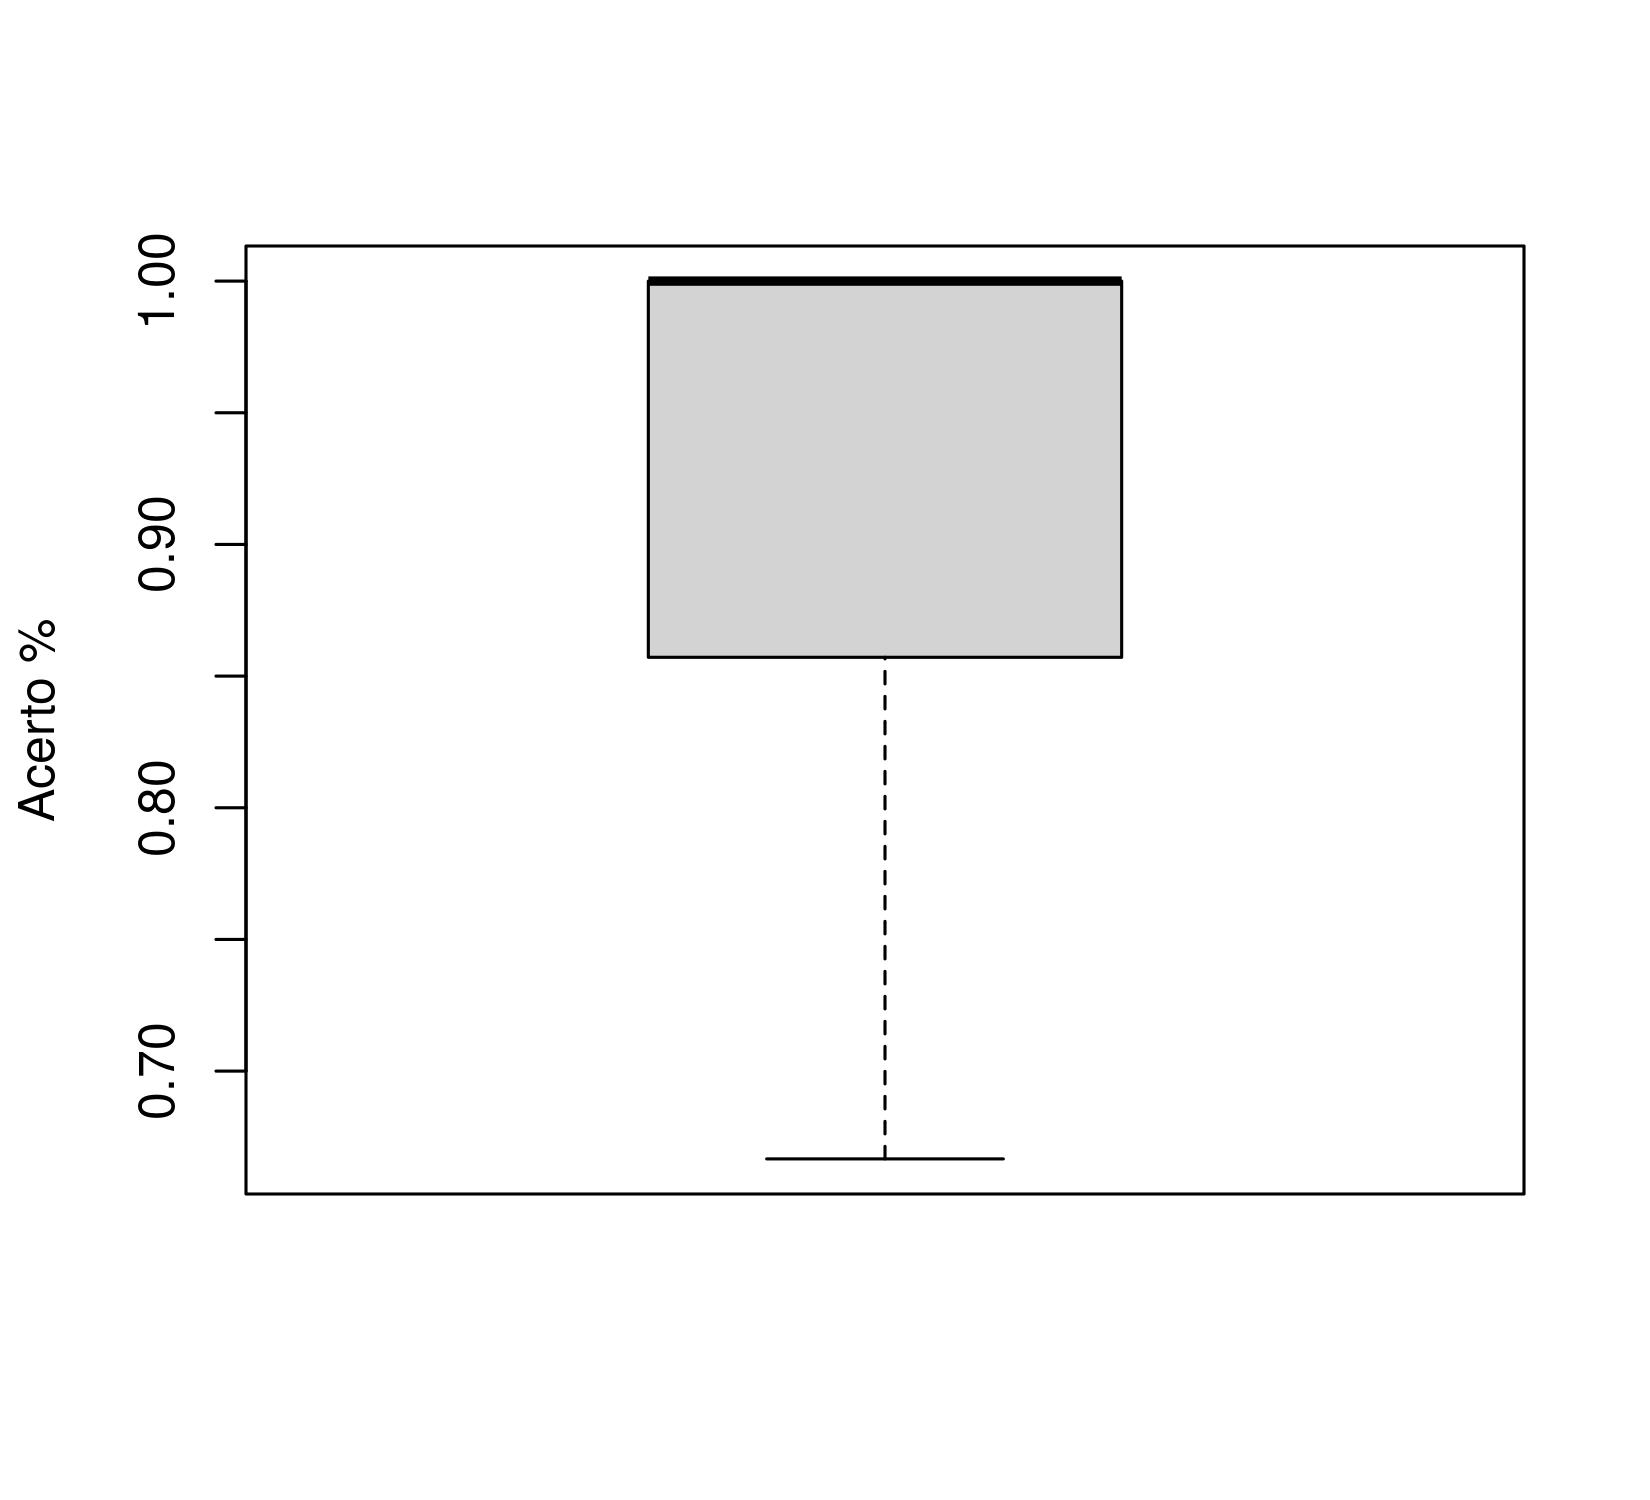
\includegraphics[width=\linewidth/2]{bar-greedy-ac-r}
\caption{RLF.}\label{fig:bar-greedy-ac-r}
\end{subfigure}
\caption{Taxa de acerto das heurísticas, diagrama de caixa.}\label{fig:barplot-greedy}
\end{figure}
\end{center}

Na tabela \ref{tab:org9793e95} é possível ver o comportamento do erro dos algoritmos em problemas reais. O algoritmo DSatur se destacou em relação a taxa de acerto que apresenta, porém assim como ele tem o menor erro também possui a pior solução porém na média isso se torna irrelevante devido a seu desempenho ótimo. Mas na média o algoritmo RLF também não fica tão atrás do DSatur. Porém é importante salientar que o algoritmo DSatur melhora muito sendo aplicado em problemas reais, ou pelo menos em problemas de certo tipo.

\begin{table}[htbp]
\centering
\begin{tabular}{lrrrrr}
Base & RLF cores & DSatur cores & \(\chi\{G\}\) & RLF Erro & DSatur Erro\\
\hline
homer & 14 & 13 & 13 & 0.92857143 & 1\\
le450\_25a & 30 & 25 & 25 & 0.83333333 & 1\\
miles500 & 21 & 20 & 20 & 0.95238095 & 1\\
miles750 & 35 & 31 & 31 & 0.88571429 & 1\\
mulsol.i.1 & 49 & 49 & 49 & 1 & 1\\
mulsol.i.2 & 31 & 31 & 31 & 1 & 1\\
queen11\_11 & 17 & 18 & 11 & 0.64705882 & 0.61111111\\
queen13\_13 & 21 & 23 & 13 & 0.61904762 & 0.56521739\\
\hline
Média &  &  &  & 0.85826331 & 0.89704106\\
\end{tabular}
\caption{\label{tab:org9793e95}
Eficiência da heurística em problemas variados. \cite{instancesgraphcoloring}}

\end{table}

Um outro fator que será comprovado empiricamente são os casos de soluções ótimas dos algoritmos.
\begin{table}[htbp]
\centering
\begin{tabular}{lrrrrr}
\hline
Tipo do grafo & V & E & \(\chi\{G\}\) & solução DSatur & solução RLF\\
Roda & 10 & 18 & 4 & 4 & 4\\
Bipartido & 10 & 9 & 2 & 2 & 2\\
Ciclo & 15 & 15 & 3 & 3 & 3\\
Ciclo & 4 & 4 & 2 & 2 & 2\\
Roda & 4 & 6 & 4 & 4 & 4\\
Bipartido & 5 & 7 & 2 & 2 & 2\\
\hline
\end{tabular}
\caption{\label{tab:orgff496a1}
Soluções em casos ótimos.}

\end{table}

\section{Conclusão}
\label{sec:org2909720}

Com esse trabalho foi possível observar a intratabilidade de um problema NPC na prática, com as análises de gráficos e regressões dos algoritmos a solução exata se mostrou inaplicável para problemas sequer de tamanhos médios. Porém isso tudo depende da quantidade de arestas no grafo, a variação dos algoritmos em relação a quantidade de arestas também foi analisada, em certas quantidades de arestas pode-se esperar que o algoritmo \emph{branch and bound} seja mais rápido que o usual.

As heurísticas propostas demonstraram grande taxa de acerto, o algoritmo RLF com grande acerto para entradas aleatorizadas e o algoritmo DSatur obtendo a solução ótima muitas vezes em problemas reais.

O algoritmo \emph{branch and bound} foi atribuído uma complexidade assintótica \(O(V^V)\), na prática a regressão obteve uma complexidade menor o que comprova que o algoritmo \emph{branch and bound} é melhor que as soluções triviais de algoritmos exatos. O algoritmo RLF foi também melhor na prática assim como o \emph{branch and bound}, se comportando com uma complexidade de \(O(V^2)\) enquanto tinha sido obtido sua complexidade \(O(V^3)\). O algoritmo DSatur foi exatamente como esperado, a complexidade obtida foi comprovada e ele foi o algoritmo mais rápido obtido com complexidade assintótica \(O(V^2)\).

A complexidade de espaço dos algoritmos foram comprovadas empiricamente e seus fatores são extremamente iguais, logo nenhum algoritmo se sobressai expressivamente nesse quesito. Então em uma abordagem prática para ver qual algoritmo aplicar iria-se estudar a quantidade de arestas em relação ao total possível e ver se há a possibilidade de aplicar o força bruta, quando não estiver perto de uma porcentagem de arestas de 87\%. Se o força bruta for inviável a escolha da heurística se dará simplesmente por qual área cada uma é melhor, o observado nos resultados é que o RLF será aplicado para problemas com natureza aleatória e o DSatur para problemas com alguma ordem.


\bibliographystyle{plain}
\bibliography{doc}
\end{document}
